\section{Conclusion}

\begin{frame}
	\frametitle{Conclusion}
	
	\begin{itemize}
		\item An overview of geometric and passivity based control methods
		\item General frameworks - application opportunities
		\item ???
	\end{itemize}
\end{frame}

\begin{frame}
	
\end{frame}

\begin{frame}
	\frametitle{Future Work (2)}
	\begin{itemize}
		\item Autonomous Wind-Turbine Blade Inspection
	\end{itemize}
	
	\begin{columns}
	
		\begin{column}{0.5\textwidth}\centering
			\begin{figure}[H]
				\centering
				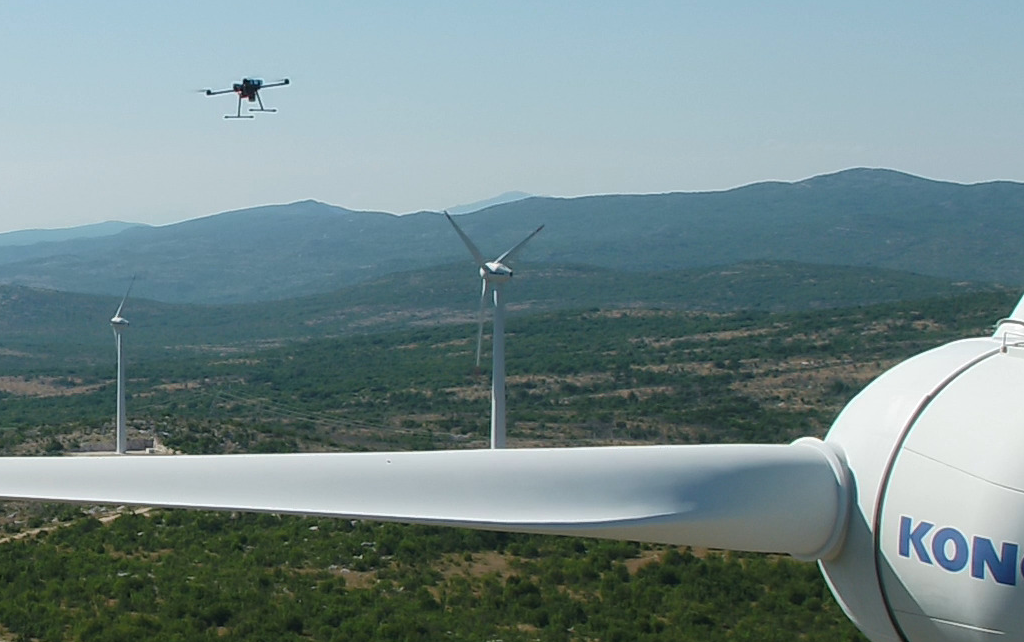
\includegraphics[width=\columnwidth]{figures/drone_flight3_1.png}
				\caption{UAV equipped with a Velodyne VLP-16 LiDAR while performing a manually operated inspection.}
			\end{figure}
		\end{column}
	
		\begin{column}{0.5\textwidth}\centering
			\begin{figure}[H]
				\centering
				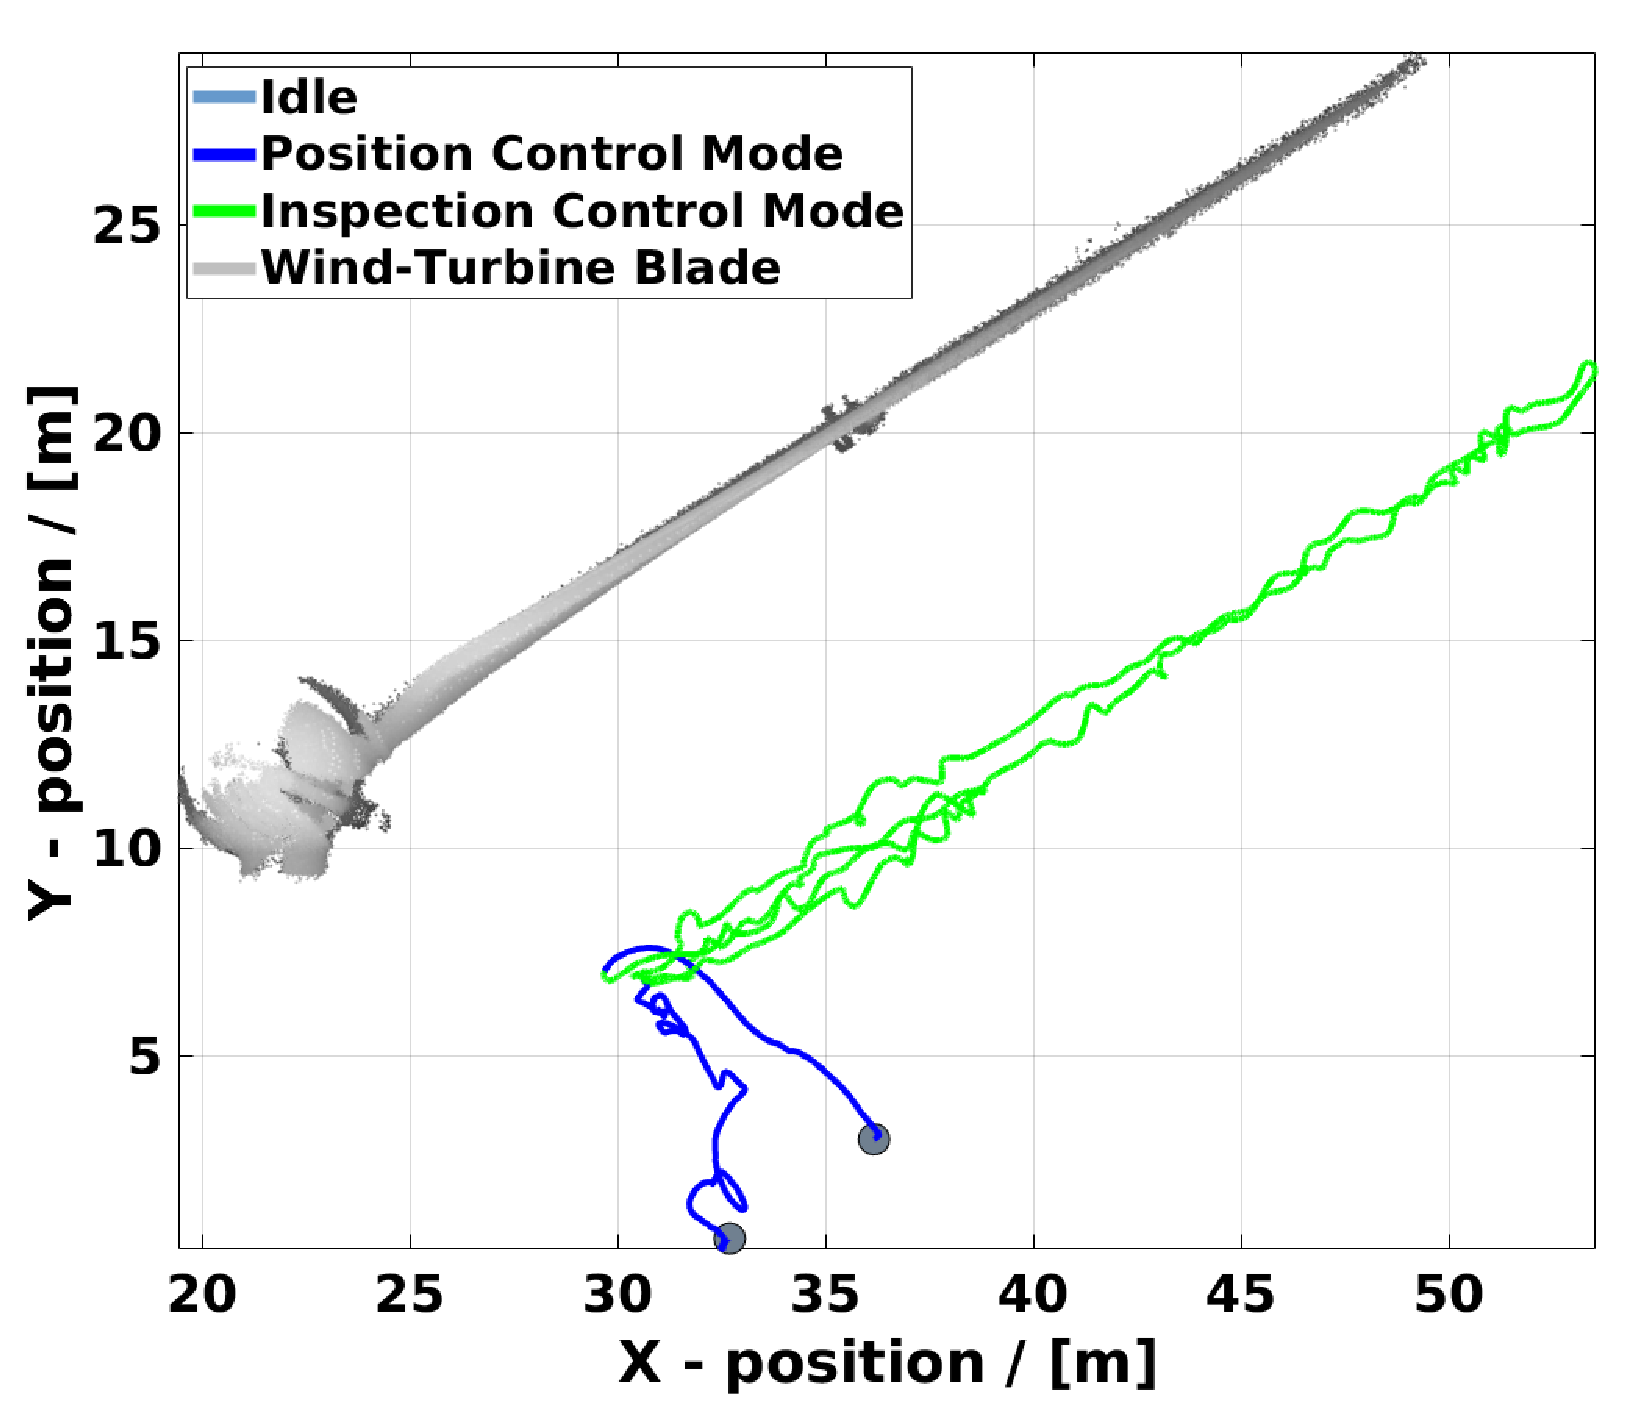
\includegraphics[width=0.9\columnwidth]{figures/uav_position_experiment_resized.pdf}
				\caption{Inspection trajectory and a wind-turbine model.}
				%\caption{Local position trajectory during the experimental wind-turbine blade inspection scenario \hlrevtwo{obtained from GPS measurements}. Blue and green colored trajectories show pilot-controlled position mode % and autonomous inspection control mode respectively. Slate gray colored markers represent takeoff and landing positions. \hlrevtwo{Wind-turbine blade model obtained post-inspection is shown as a reference.} }
			\end{figure}
		\end{column}
	\end{columns}
\end{frame}

\begin{frame}
	\frametitle{Future Work (3)}
	\href{video_presentation.mp4}{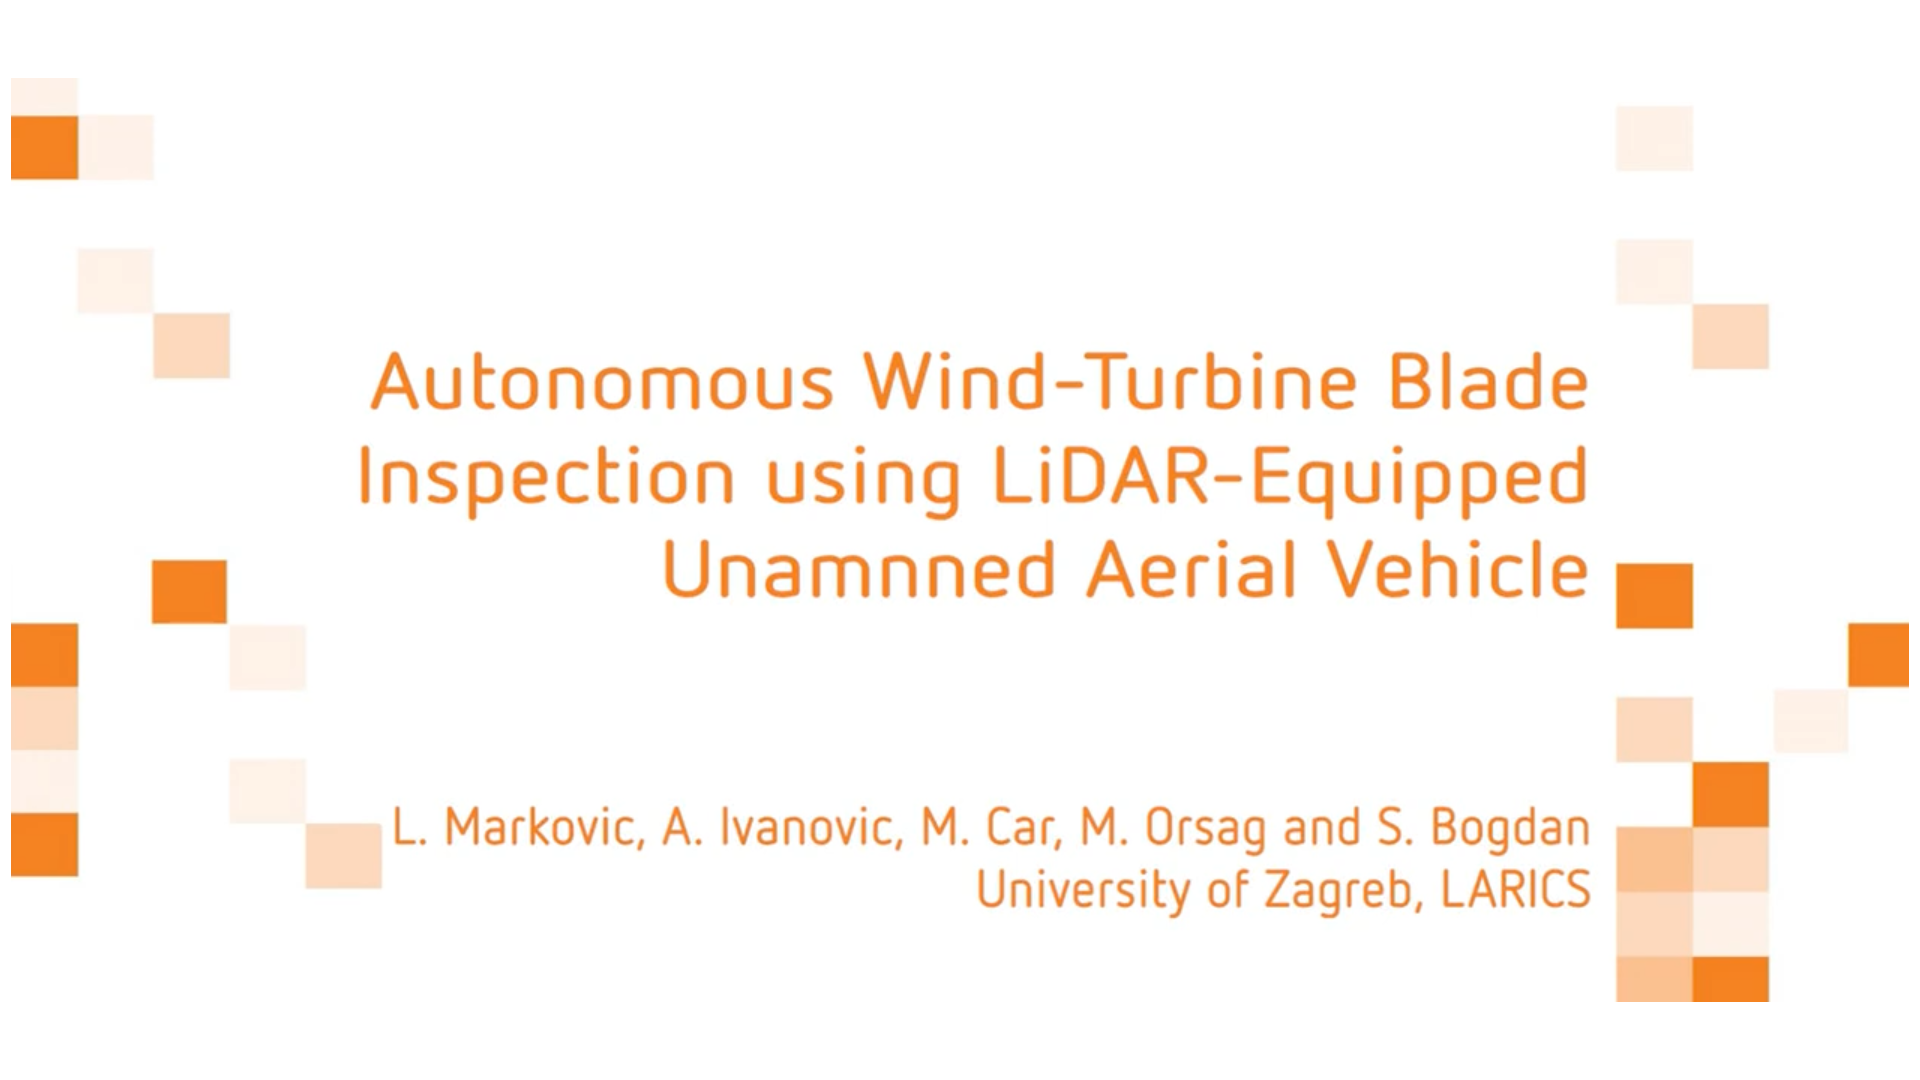
\includegraphics[width=\textwidth]{figures/title_screen.png}}
\end{frame}
